\documentclass{article}
% The preceding line is only needed to identify funding in the first footnote. If that is unneeded, please comment it out.

\usepackage[preprint]{jmlr2e}

\usepackage{amsmath,amssymb,amsfonts}
\usepackage{algorithmic}
\usepackage{graphicx}
\usepackage{textcomp}
\usepackage{xcolor}

\DeclareMathOperator*{\argmax}{arg\,max}
\DeclareMathOperator*{\argmin}{arg\,min}

\binoppenalty=\maxdimen
\relpenalty=\maxdimen

\def\BibTeX{{\rm B\kern-.05em{\sc i\kern-.025em b}\kern-.08em
    T\kern-.1667em\lower.7ex\hbox{E}\kern-.125emX}}

% Short headings should be running head and authors last names

\ShortHeadings{Sparse, Smooth and Differentiable Hyperspectral Unmixing}{Aymeric CÔME  \& Pierre-Antoine THOUVENIN}
\firstpageno{1}

\begin{document}

\title{Sparse, Smooth and Differentiable Hyperspectral Unmixing using Dispersion Model}

\author{\name Aymeric CÔME \email aymeric.come.etu@univ-lille.fr \\
       \addr Master Data Science\\
       University of Lille, Centrale Lille, IMT Lille-Douai\\
       Villeneuve d'Ascq, France
       \AND
       \name Pierre-Antoine THOUVENIN \email pierre-antoine.thouvenin@centralelille.fr \\
       \addr Assistant professor and member of SigMA team\\
       Université de Lille, CNRS, Centrale Lille, CRIStAL\\
       Villeneuve d'Ascq, France}

\maketitle

\begin{abstract}%
  Hyperspectral unmixing consists in infering the proportion of presence (\emph{abundance}) and \emph{signatures} of pure materials composing an hyperspectral image, observed over hundreds of wavelengths. The spectra observed in each pixel indeed result from a mixture of several signatures, referrend to as \emph{endmembers}, which characterize the materials present in the observed scene. The problem is challenging in that it is not only non-linear, but can be further affected by multiple factors which can locally affect the shape of the endmembers, the so-called spectral variability. To tackle this problem, \citet{janiczek_differentiable_2020} introduced a physics-based, differentiable model to realistically capture endmembers. However, the approach investigated in \citet{janiczek_differentiable_2020} exploits none of the usual prior information commonly used in the literature (e.g. spatial smoothness, sparse abundances). In this project, we propose to extend this approach by considering additional regularization terms on both the abundances and the variability, and investigate their impact on unmixing quality.
\end{abstract}

\begin{keywords}
Hyperspectral Unmixing, Linear Unmixing, Differentiable Programming, Endmember Spatial and Spectral Variability
\end{keywords}

\section{Introduction}
In many real-world applications such as astronomy \citep{kouyama2016}, remote sensing \citep{lu_2014} or mineral detection \citep{bandfield2002}, hyperspectral images (which consist of samples of electromagnetic spectra at various wavelengths) can put into evidence some key characteristics of the location monitored. In particular, it is commonly assumed that each physical material present in the scene, called endmember (EM), have its own signature spectrum, which contributes to the HI, depending on its proportion of presence in each pixel. Hence, recovering these characteristic signatures from HI leads to a precise description and detection of materials in a scene.

However, despite the high spectral resolution of hyperspectral cameras, technical limits must be taken into account; for instance a limited spatial resolution or a varying luminosity can be expected. This implies that the pixels of a HI then contain mixtures of multiple EMs in varying abundances, and noise is injected into the measurement. That means that the signature spectra of EMs can vary spectrally and spatially. While many unmixing algorithms have already been proposed \citep{borsoi_spectral_2020}, the physics behind is often too complex to be fully modelled or the physical quantities at hand are unknown.

A first difficulty to handle is the spectral variability (SV): depending on the scene observed, an EM might have a signature different from a laboratory measurement. This kind of variability can even occurs locally, between pixels of a same HI, which actually question the hypothesis of one reference signature characteristic of one EM, rather than a class of signatures. Multiple factors can contribute to this variability, and we distinguish two kinds: intrisic and external. Intrisic variability is due to the natural differences of the EM samples across the HI (e.g. grass is greener on the other side because the neighbor water it) while external variability refers to the environment influence, like light and shade or the quality of the hyperspectral camera used.

In the end, hyperspectral unmixing is very challenging task in that there are many unknowns and sources of variability, hence it requires prior information to regularize the problem and improve the inference process.

Linear Mixing Models \citep{LMM} are a classic approach to model mixture spectra as a linear combination of the reference signatures and the abundances, plus some noise. To handle spectral variability, different signatures across the pixels of the HI can be considered. Moreover, multiplicative \citep{veganzones2014} or additive \citep{johnson2013} variability of the spectra have been studied in the literature. An other approach is to perform a physical analysis of the context, to try to provide an explicit model of spectral variation \citep{janiczek_differentiable_2020,griffin2003}. And lately, Deep approaches have been tested \citep{borsoi_deep_2019}.\\

\textbf{Contributions:}
In this report, we propose to take advantage of the physics-based dispersion model introduced in \citet{janiczek_differentiable_2020} in order to perform spectral unmixing. More precisely, we incorporate important prior information about the elements of the problem (such as sparsity of the abundances or spatial smoothness for the EMs) that should improve the regularisation of the problem, and then we present a new formulation of the unmixing problem. Additionally and in the same fashion as in \citet{janiczek_differentiable_2020}, we keep the problem differentiable to exploit on-the-shelf algorithms, with automatic differentiation because of the complexity of the dispersion model. Finally, we run some experimentations on real-world and synthetic data, to validate the approach.\\

The report is organised as follows. A brief summary of different approaches to endmember variability modelling is given in section REF(SECTION). Section REF(SECTION) is devoted to the formulation of the problem, introducing the a priori information considered to solve the problem. The algorithm used to address the resulting optimisation problem is briefly described in Section REF(SECTION). Experiments reported in Section REF(SECTION) propose a first validation of the approach on synthetic data. Conclusion and perspectives are finally reported in Section REF(SECTION).

\section{Variability models}
In this section is presented a quick review of the literature on variability models for HI. In these applications, it is commonly assumed that the target mixture spectrum is a function of the signature spectra of the EMs present in the scene, and their abundances. Moreover, and we make this hypothesis in our contribution as well, the number of EMs is supposed to be known a priori - there exist many state-of-the-art algorithms to try to infer this information \citep{bioucas2008}. Now the following models are designed specifically to consider SV.

\subsection{Generic explicit models}
The Linear Mixture Model (LMM) is defined as follows:
$$y_n = M_0 a_n + z_n$$
for a pixel $n$ of an HI. $M_0$ is a $S \times P$ matrix whose columns correspond to the signatures of the $P$ EMs, over the $L$ spectral channels, and $a_n$ is a $P$ vector, giving for each EM its abundance in the pixel (so that the elements of $a_n$ are non-negative and sum to $1$). $z_n$ is additive noise. The main culprit of this model that has been demonstrated is the proportion indeterminancy \citep{borsoi_spectral_2020}.

To consider spatial variability of the EMs, often a varying matrix of signatures is studied:
\begin{equation}\label{eq:LMM}
  y_n = M_n a_n + z_n
\end{equation}
Now the signatures of the EMs depend on the pixel, hence on the spatial location. However, the difficulty is to express $M_n$. Multiple approaches have been proposed to do so. Some are based on spectral libraries, consisting on trying to match reference signatures to the observations. Others create such libraries directly from the image, using pure pixels (only one EM present) for instance.

\subsection{Deep models}
While previous methods have shown good performances, they often depend on expensive and not always available previous informations about the EMs. Since the problem seems too complex to be described by simple models, the scientific community has designed Deep architextures, that could learn in a black-box manner the rules underlying spectral variability.

In \citet{borsoi_deep_2019}, the authors train a Variational Auto-Encoder that learns a latent representation of EM signatures, which is then used in a classic LMM optimisation framework. In particular, this works is based on the smoothness of the latent space; we will use a similar hypothesis later on as well. Yet, the method once again requires a pure pixels or libraries for training.

Another Deep approach is deployed in \citet{hong_endmember-guided_2021}: one neural network is used to learn a relevant representation of EMs signatures, and at the same time guide an unmixing network through weight sharing. Once again, this approach makes use of pure pixels in the HI. More interestingly, the networks use the convolution operation: the spatial correlation between pixels is used to perform unmixing.

Finally, the work presented in \citet{feng_hyperspectral_2018} leverages matrix factorization with Deep networks. The observed HI is supposed to be decomposable as a successive multiplication of matrices, the last one being the abundance map, each previous matrix represented by a layer in the neural network. A major point of this approach is the addition of a sparsity penalty in the loss function: the factorization is supported by a sparsity regularization on the abundances.

Thus, Deep approaches to generate variable signatures encounters some succes; however the training can be difficult, and often require prior information to converge to a good solution.

\subsection{Physics-based models}\label{sec:dispersion}
So far have been presented generic or Deep models for the variable signatures $M_n$ (\ref{eq:LMM}). An interesting observation is the use of prior information about the structure and behavior of the elements of the problem, to regularise and help the algorithm find a good solution.

A last strategy to model the SV are physics-based models: an explicit description of the signatures derived from physical laws. This can be compared to the VAE, in that it is a mapping of signatures to a latent space of parameters controlling their generation, based on the current state.

\citet{janiczek_differentiable_2020} presents such a model, the dispersion model, derived from the laws behind molecular vibration. Then the optimisation problem consist in infering the parameter values for each EM, and then generate the corresponding signature and unmix the target HI in accordance with the LMM model (\ref{eq:LMM}). One important property of the dispersion model is that it is differentiable, which allows for an easier optimisation algorithm.

In the dispersion model, every EM is characterized by a set of parameters $\rho, \omega_0, \gamma, \epsilon_r \in \mathbb{R}^K$ (band strength, resonant frequency, frictional force, relative dielectric permeability), where $K$ is an hyper-parameter corresponding to the number of equations controlling the signature, and for every such equation ($k$) are involved $\rho_k, \omega_{0, k}, \gamma_k, \epsilon_{r, k}$ in a very complex - but differentiable - way. Then, the spectral emission of the Em can be computed for every wavelength $\omega$: $\widehat\epsilon(\theta; \omega)$, where $\theta$ is the matrix of parameters. We denote by $E(\theta_1, \dots, \theta_P) \in \mathbb{R}^{S \times P}$ the matrix whose columns contain the spectral signature over the $S$ wavelengths considered, for all $P$ EMs.

Following the LMM (\ref{eq:LMM}), the authors formulates the unmixing problem as:
\begin{equation}\label{eq:dispersion}
  \argmin_{\theta_{min} < \theta < \theta_{max},\ a} \| b - E(\theta_1, \dots, \theta_P) a \|_2^2 + \lambda \| a \|_p
\end{equation}
where $b$ is the spectra at one pixel of the HI, $a$ is the vector of abundances (non-negative, sum to one), and a regularisation term to promote abundance sparsity with a pseudo-norm $p < 1$.

The algorithm proposed, called \emph{Analysis-by-Synthesis}, solves (\ref{eq:dispersion}) for every pixel. To do so, an alternating-like minimisation is performed: at each iteration the objective function is minimized on $a$ only, then an gradient descent update of the parameters $\theta$ is done, using the chain rule to backpropagate the gradient up to the parameters (thanks to the differentiability of the dispersion model).

To avoid falling into a bad local minimum, the authors support that a good initialisation is provided by fitting each EM separately to $b$. This abides by the sparsity assumption made on the abundances.

In the end, the dispersion model seems to provide a good model for the EMs, and has the upside of being differentiable. However, no spatial correlation is used, and the alternating minimisation isn't justified theoretically. Hence, we come up with an other optimisation framework for performing hyperspectral unmixing with the dispersion model: the next section present it.


\section{Problem statement}
Based on the elements and observations we have seen so far, we come up with a formulation for the problems we are willing to tackle.

\subsection{Reconstruction model}
The first part of a spectral unmixing strategy is to try to reconstruct the target HI from a specified observation model, which describes the relationship between the observations and the parameters to be inferred.

In this work, we propose to make use of the dispersion model presented in Section \ref{sec:dispersion}. So, the reconstructed spectra are generated by the dispersion model from the physics parameters. More precisely, we suppose that each EM is present in a state characterised by those parameter values in every pixel; and then each EM is associated to a signature spectrum derived from the dispersion model. The SV is modeled here by the variation of the parameter values through the HI, which in turn gives different signature spectra over the pixels. Regarding the unmixing, we decided to use Linear Unmixing once again, so that our model would still compare to the one in the original paper. We then introduce abundances for each EM, accross the HI.

\subsubsection{Problem statement}

We consider a HI $B \in \mathbb{R}^{N \times M \times S}$ consisting of $N \times M = L$ pixels, each pixel giving a spectrum evalutated at wavelenghts $w_1,\dots, w_S$. We assume that there are $P$ EMs in the HI, characterised by sets of vectors of parameters $\theta_1,\dots, \theta_P$.

Since the dispersion model from \citet{janiczek_differentiable_2020} is adopted here, the parameters $\theta_p \in \mathbb{R}^{N \times M \times K \times 4}$ contain the physical parameters introduced in the previous section REF(SECTION), with different values for different pixels (for sake of lisibility, we define $T = K \times 4$ the number of parameters per EM).

Then, the corresponding abundance map $A \in [0, 1]^{N \times M\times P}$ is such that $a_{i, j, p}$ is the abundance of EM $p$ in pixel $(i, j)$, and $\|A_{i, j, 1:P}\|_1 = 1$.

Finally, $E(\theta_1,\dots, \theta_P) = E(\Theta) \in \mathbb{R}^{N \times M \times P \times S}$ holds the signature spectrum of each EM at each pixel, derived from the dispersion model: $E(\Theta)_{i, j, p, s} = \epsilon(\theta_{i, j, p}; w_s)$.

\subsubsection{Model of the hyperspectral image}

In accordance to a commonly used approach in the literature ADD CITATION, we model the HI as follows:
$$B = E(\Theta) A + Z$$
where $Z$ is a white noise tensor and $E(\Theta) A \in \mathbb{R}^{N \times M \times S}$ is the sum of the signature spectra weighted by abundances, for every pixel and spectral channel.

So far it is just a reformulation of the problem from \cite{janiczek_differentiable_2020}, however we wish to add prior information on the elements of the problem, as discussed in the following sections. This will be expressed by additional terms in the objective function. In the end, the optimisation problem states as:

\begin{equation}
  \label{eq:objective}
  \argmin_{\Theta \in \Delta,\ A \in \Upsilon} H(\Theta, A) + f(\Theta) + g(A)
\end{equation}
with $H(\Theta, A) = \frac{1}{2 L} \|B - E(\Theta) A\|^2$, and $\Upsilon$ and $\Delta$ are constraint spaces presented afterwards. The norm used on tensors, defined by $\|Q\| = \sqrt{\sum_{1 \leq i \leq N,\\1 \leq j \leq M} \|Q_{i, j, 1:S}\|_2^2}$, is the Froebenius norm applied on the square norm over spectrum for every pixel. $f(\Theta)$ and $g(A) = g_c(A) + g_s(A)$ are regularisation terms, enforcing priors on the parameters.

This formulation corresponds to finding the maximum likelihood in presence of white noise, with respect to priors.

\subsection{Priors on the endmembers}
In this section are explained the priors introduced regarding the EMs present in the HI.

\subsubsection{Physics-based constraints}

The main prior regarding EMs is that they follow the physics-based dispersion model, controlled by the parameters $\Theta$. These parameters actually represent physical quantities (frictional force, band strength...): in that regard, and alike what was done in \cite{janiczek_differentiable_2020}, their values should stay in a plausible range, determined by a physical analysis. From now on, we will design by $\Delta$ the space in which the parameters $\Theta$ live:
$$\Delta = [\rho_{min}, \rho_{max}] \times [\omega_{0, min}, \omega_{0, max}] \times [\gamma_{min}, \gamma_{max}] \times [\epsilon_{r, min}, \epsilon_{r, max}]$$

\subsubsection{Smoothness}\label{sec:EM-smoothness}

As advertised earlier, our approach to model the SV is to let the physical parameters $\Theta$ of the EMs vary across the pixels of $B$. Yet, to keep a spatial consistency we want to ensure a smooth variation, to represent the idea that, as the environmental conditions are roughly continuous with respect to space dimensions, so are material states and signature spectra. For instance, the quantity of water received by a lawn is close to the one received by the adjacent grass. Obviously, this hypothesis is not always appropriate, as your neighbor might water his lawn way more than you; yet it should still be a relevant hypothesis in most real-world applications ADD CITATION.

To do so, we consider the \emph{discrete gradient} operator, as in \citet{condat_generic_2014}. It consists in the horizontal and vertical differences between neighbour pixels, so that for an $N \times M$ image $Y$ we have:

\begin{align*}\label{eq:discrete-grad}
  D(Y) &= (u_h (Y),\ u_v (Y)),\\
  u_h (Y) [i, j] &= Y_{i+1, j} - Y_{i, j} \text{ if }i + 1 \leq N,\ 0 \text{ otherwise}\\
  u_v (Y) [i, j] &= Y_{i, j+1} - Y_{i, j} \text{ if }j + 1 \leq M,\ 0 \text{ otherwise}
\end{align*}

This operator is a measure of the spatial variation of the pixel values, hence in order to promote smoothness these differences should remain small. We quantify it with:

\begin{align*}
  \| D(Y) \|_{1,2} = \sum_{i=1}^N \sum_{j=1}^M \sqrt{ u_h (Y)[i, j]^2 + u_v (Y)[i, j]^2 }
\end{align*}

Finally, we enforce smoothness by minimizing the sum of the squared variations, so that the corresponding term is (for some penalty factor $\gamma >0$):

\begin{align}\label{eq:f}
  %f(\Theta) &= \gamma \mathcal{L}(\Theta)\\
  f(\Theta) &= \gamma \sum_{t = 1}^{T} \sum_{p = 1}^P \| D(\Theta_{:,:,p,t}) \|_{1,2}^2
\end{align}

Note that one might prefer to ensure smoothness of the spectra rather than the parameters; we would then have:
\begin{align*}
  f(\Theta) &= \gamma \sum_{t = 1}^{T} \sum_{p = 1}^P \| D(E(\Theta_{:,:,p,t})) \|_{1,2}^2
\end{align*}

\subsection{Priors on the abundances}
We introduced the material abundances of each EM in every pixel, and, in accordance with the Linear Unmixing Model, we assume that an EM contributes to the mixture signal proportionally to its abundance. To stay in a relevant case, we need to ensure that some properties are respected for the abundances.

\subsubsection{Constraints}

Based on their physical meaning, abundances of EMs must obviously be positive and sum to 1 in each pixel. These constraints are usually formulated using an indicator operator:

$$\iota_\Upsilon (A) = \begin{cases} 0 \text{ if A}\in \Upsilon\\ +\infty \text{ otherwise} \end{cases}$$
where
$$\Upsilon = \{Q \in \mathbb{R}^{L \times P}_+\ |\ \| Q_{i, j, 1:P} \|_1 = 1 \ \forall 1 \leq i \leq N, 1 \leq j \leq M\}$$
is the simplex where abundances live.

However, constraints induce non-differentiability. To circumvent this issue, we propose to relax the constraint term into a smooth penalty term, so that we strongly encourage abundances to stay close the $\Upsilon$ while being differentiable.

The idea is to strongly promote values close to $\Upsilon$ for $A$, thanks to an approximation to the indicator function. Such approach has already been presented and used in the literature, in the form of \emph{log-barrier method} ADD CITATION. In particular, we consider the \emph{log-barrier extension} introduced in \citet{kervadec_constrained_2020}. This operator is convex, continuous and twice-differentiable, and is defined as follows, for some hyper-parameter $t > 0$:
$$\forall z\in \mathbb{R},\ \tilde\Psi_t (z) = \begin{cases} - \frac{1}{t} \log (-z) & \text{if } z \leq -\frac{1}{t^2}\\ tz - \frac{1}{t} \log(\frac{1}{t^2}) + \frac{1}{t} & \text{otherwise} \end{cases}$$

The higher $t$, the better the quality of the approximation; however one should be cautious not to overwhelm the other terms in the problems - this is discussed the next section.

To translate the sum-to-one constraint on the abundances, we rewrite it as a sum-greater-than-one and sum-lesser-than-one constraint, in addition to the positivity constraint. Finally, we come up with the following penalty term, $\zeta > 0$ and $\nu > 0$ being hyper-parameters:
\begin{equation}\label{eq:g_c}
  g_c (A) = \zeta \cdot \Bigg[ \sum_{i = 1}^N \sum_{j = 1}^M \sum_{p=1}^P \tilde\Psi_\nu (-a_{i,j,p}) + \sum_{i = 1}^N \sum_{j = 1}^M \left[ \tilde\Psi_\nu(\sum_{p=1}^P a_{i,j,p} - 1) + \tilde\Psi_\nu(1 - \sum_{p=1}^Pa_{i,j,p}) \right] \Bigg]
\end{equation}

\subsubsection{Sparsity}

Regarding the abundances, we whish to enforce sparsity of abundances in every pixel; we would rather have a few EMs in significant abundances than a lot of EMs in small quantities. This prior is often relevant in real-wolrd applications ADD CITATION.

Common choices to do so are the $\ell_0$ count measure, the $\ell_1$ norm, or the $\ell_p \ (p<1)$ quasi-norm ADD CITATION. However, these terms are hard to handle during optimisation, as they introduce non-convexity and discontinuity. Hence, to keep once again our problem differentiable, we ressort to the SPOQ regularisation, introduced in \citet{cherni_spoq_2020}. It gives a smooth approximation of $\ell_0$.

For some hyper-parameters $p\in \, ]0, 2[$, $q\in \, [2, +\infty[$, and $(\alpha, \eta) \in \, ]0, +\infty [^2$, the SPOQ regularisation term is defined as follow, for any vector $x \in \mathbb{R}^N$:
$$SPOQ(x) = \log \left( \frac{(\ell_{p,\alpha}^p (x) + \beta^p)^{1/p}}{\ell_{q,\eta} (x)} \right)$$
        where
        $$\ell_{p,\alpha} (x) = \left( \sum_{n=1}^N (x_n^2 + \alpha^2)^{p/2} - \alpha^p \right)^p$$
        $$\ell_{q,\eta} (x) = \left( \eta^q + \sum_{n=1}^N |x_n|^q \right)^{1/q}$$

The choice of the hyper-parameters is discussed in the next section.

We then apply the SPOQ pseudo-norm on the vector of abundances in every pixel of the HI:
$$SPOQ(A) = (SPOQ(a_{i,j,1:P}))_{i, j} \in \mathbb{R}_+^{N \times M}$$

In the end, we define the sparsity term on abundances as (with $\delta > 0$ a penalty term):
\begin{equation}\label{eq:g_s}
  g_s(A) = \frac{\delta}{N \times M} \| SPOQ(A) \|_{1}
\end{equation}

It simply is a sum of the SPOQ norms over the pixels.

\subsubsection{Smoothness}
Finally, one could also require the abundances to vary smoothly across space. Hence, in a similar way to Section \ref{sec:EM-smoothness}, we could add a $\beta \mathcal{L}(A)$ term to the regularisation on abundances. We will not consider it here though, for simplicity and because we value the sparsity prior more.


\section{Inference algorithm}

The optimisation problem presented in (\ref{eq:objective}) is composed of one differentiable, non-convex block $H(\Theta, A) + f(\Theta)$ and one non-convex, non-continuous block $\delta\|A\|_{1,0} + \iota_\Upsilon (A)$, and deal with two vectors of parameters $\Theta$ and $A$.

The first alternative to non-differentiability is to use Moreau's proximal operator: a first-order approximation of a gradient descent step. We would then operate an alternating minimization on $\Theta$ (differentiable) and $A$ (non-differentiable). However, algorithms involving this operator typically rely on the knowledge of a (tight) Lipschitz constant of the differentiable part to derive a fitting learning rate, and due to the complex definition of the dispersion model we do not have access to such a constant. Moreover, one can't easily derive the close form of the proximal operator of an addition of two non-differentiable, non-convex terms.

Related families of optimisation algorithms would be subgradient or bundle algorithms, unfortunately they do not seem to apply to our problem, mainly because of the non-convexity and the fact that in the constraint $\iota_\Upsilon$ on $A$, $\Upsilon$ is a simplex rather than a convex space.

Hence, instead of testing such approaches without guarantees, we chose a Lagrangian-based method from Kervadec2020, using a \emph{log-barrier extension} to replace the constraint term for $A$. Then, thanks to Cherni2020 we approximate the sparsity term on $A$ with a smooth approximation, so that as written in (\ref{eq:general}) we put ourselves in a smooth context.

Finally, thanks to these rewritings we are able to do a Stochastic Gradient Descent-like optimisation with Adam-which has already shown to be an efficient approach for such problems. A discussion can be made on other Adam-like algorithms in a non-convex problem (cf Chen2019), yet we will stick to the classical Adam for simplicity reasons. In particular, we shall use the Autodiff feature from PyTorch rather than deriving by hand the awfully complex gradient of (\ref{eq:general}).

To wrap-up, the inclusion of our priors raised some major optimisation issues, due to which we have been forced to resort to a sub-optimal approach. Hopefully, the behavior will still be good, thanks to the senseful priors and a good initialization provided by the dispersion model. On the other hand, Janiczek \emph{analysis-by-synthesis} consists in an alternating minimization of the reconstruction error, on the abundances and the physics parameters. The main difference with our approach is that the parameters (and then the signature spectrum) of EMs are assumed to be the same all accross the HI.

\section{Experiments}
In order to validate our approach, we implemented it using \textsf{PyTorch} \footnote{https://pytorch.org/} with \textsf{Python 3.7}; the details can be found on GitHub \footnote{https://github.com/Javisty/spectral\_
unmixing}. In this section we describe the data used, the evaluation process, and make some discussion and comparison with \citet{janiczek_differentiable_2020}, before presenting and analysing the results.

\subsection{Experimental settings}
\subsubsection{Datasets}
Ideally we would experiment on multiple real-world datasets for which we have access to the ground-truth abundance map and EM parameters and signature spectra in addition to a 2D HI, however such data is very hard to obtain. Additionaly, we should compare our performances with the ones of \citet{janiczek_differentiable_2020}. Hence we resort to one dataset used in \citet{janiczek_differentiable_2020} and one synthetically generated.

\textit{Feely et al. dataset \cite{feely}:} 90 samples of thermal emission spectra in the infrared for various minerals measured in the lab, over $830$ spectral channels. Ground truth was determined via optical petrography, and a labeled endmember library is provided, so that we have the true abundances for the $38$ EMs. Also, as the EMs are known minerals, we can already initialize the parameters $\Theta$ with physics-based values. \citeauthor{janiczek_differentiable_2020} already tested the dispersion model on this data, so we want to compare how our additional priors will affect the results. Unfortunately, as the samples are actually independent pixels, we couldn't use spatial regularisation here.

\textit{Synthetic data \cite{thouvenin}:} synthetically generated data, with white Gaussian noise (SNR=15dB) and some random SV. The HIs have size $128 \times 64$, and are generated from $3$ or $6$ EMs for $413$ spectral channels. We are able to test all our priors on this dataset, yet it is important to note that the spectra have been generated independently between the pixels, so that our spatial smoothness priors doesn't hold here. The code is available on GitHub \footnote{https://github.com/pthouvenin/synthetic-hs-variability}.

\subsubsection{Evaluation criteria:}
To assess the performance of the approach, we use some common metrics in the literature: aSAM (average Spectral Angle Mapper) and RMSE (Root Mean Square Error) for the EMs signature spectra, MSE for abundances (per EM and global) and the reconstruction error $H(\Theta, A)$.

\begin{align*}
  aSAM(\widehat{E}) &= \frac{1}{N M P} \sum_{p=1}^P arccos \left( \frac{\widehat{\epsilon}_p^T\ \bar{\epsilon}_p}{\| \widehat{\epsilon}_p \|_2 \| \bar{\epsilon}_p \|_2} \right)\\
  MSE(\widehat{A}) &= \frac{1}{N M P} \| \widehat{A} - \bar{A} \|_{\mathcal{F}}^2
\end{align*}

We shall as well compare those results with the ones of \citet{janiczek_differentiable_2020}.

\subsubsection{Compared methods:}
This work applys the dispersion model in an other optimisation framework, in which we promote sparsity of abundances and spatial smoothness in a differentiable way. Then, we solve the problem with a classic gradient descent algorithm. Of course, the objective function is strongly not convex, yet as in \citet{janiczek_differentiable_2020} we rely on a good initialisation of the EM parameters to find a relevant minimum.

On the other hand, in the reference paper they set their dispersion model in a mixed optimisation problem, between Alternating Minimization ADD CITATION and Block Coordinate Decent ADD CITATION. Indeed, in the analysis-by-synthesis at each iteration a full minimization is performed on the abundances by performing Sequential Least Squares Programming ADD CITATION, and then one step of gradient descent (Adam \citep{kingma_adam_2017}) is done on the EM parameters.

\subsubsection{Training and implementation details:}
The final model has a lot of hyper-parameters to fix: number of EMs $P$, penalty factors $\delta, \zeta...$, $SPOQ$ and log-barrier ($p, \alpha, \nu...$), Adam parameters.

The values for the SPOQ parameters were taken from \citet{cherni_spoq_2020}, Section II.B: $p=1/4$, $q=2$, $\alpha=7 \times 10^{-7}$, $\beta = 3 \times 10^{-3}$ and $\eta= 1 \times 10^{-1}$. Similarly, we imitated the approach described in \citet{kervadec_constrained_2020} (Appendix, Section E) regarding the log-barrier extension $\nu$ hyper-parameter: it is initialised at 5, and is multiplicatively increased by a factor $1.1$ between each Adam step. The authors justify this choice by saying that in the early stages of optimisation, the model needs more relaxation with respect to the constraints, and the latters are gradually enforced as the algorithm converges. In practice, during the experiments we capped its value at $1/\nu^2 = 1 \times 10^{-3}$. Indeed, the loss rapidly explodes for bigger values of $\nu$, as the algorithm isn't able anymore to minimize both $H(\Theta, A)$ while respecting the constraints on $A$ with an ever greater precision.

The Adam parameters used were a learning rate of $0.01$, and the standard values suggested by \textsf{PyTorch}\footnote{https://pytorch.org/docs/stable/generated/torch.optim.Adam.html}. The learning rate actually required some fine-tuning, as a too high value would cause the model to oscillate too much between a good reconstruction and an abundance map respecting the priors, while a low value gets the model stuck in a bad local minimum, preventing exploration.

Regarding the penalty factors, the values were chosen between $0.1$ and $1$. In particular, we made sure that the sparsity term $g_s(A)$ didn't take precedence over the constraining one $g_c(A)$, as the latter is more important.

The number of epochs before convergence were around $70$ for the Feely dataset; on the synthetic one it changed a lot for different sets of hyper-parameters.

Finally, as mentioned earlier the initialisation is an important aspect in this optimisation problem. For the Feely dataset, like in \citet{janiczek_differentiable_2020} we initialised the physical parameters with the associated EM library, which gives reference values for the materials studied. The abundance map was initialised with a homogeneous repartition. Regarding the synthetic dataset, initialisation signatures were given, so that the parameters were set by fitting these signature spectra for each EM. An initial abundance map was provided as well.

\subsection{Results and Discussion}

\begin{table}
\centering
\begin{tabular}{ccccc}
{} & {\bf aSAM(E)} & {\bf RMSE(E)} & {\bf MSE(A)} & {\bf RE} \\
\hline & \\[-1.5ex]
EM 1 & 0.337 & 0.266 & 0.120 &  \\
EM 2 & 0.634 & 0.430 & 0.163 &   \\
EM 3 & 0.547 & 0.415 & 0.0122 &   \\
EM 4 & 0.342 & 0.260 & 0.0112 &  \\
EM 5 & 0.341 & 0.411 & 0.0112 &  \\
EM 6 & 0.213 & 0.142 & 0.139 &  \\
Average & 0.403 & 0.138 & 0.0766 & 0.907 \\
\end{tabular}
\caption{Results after 1000 epochs on the synthetic dataset with 6 endmembers.}
\label{table:results-6}
\end{table}

\begin{figure*}[!t]
    \centering
    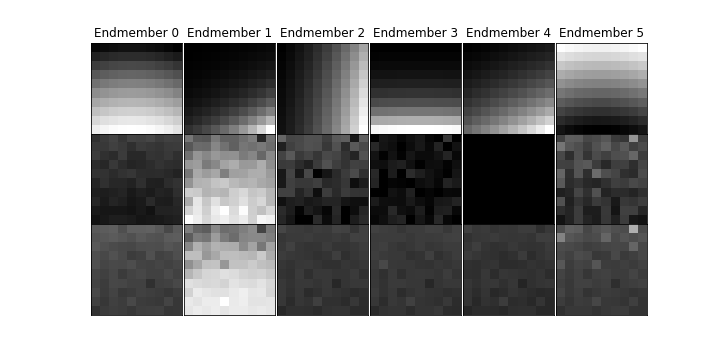
\includegraphics[width=\textwidth]{pictures/abundance_maps.png}
    \caption{Truth, initial and predicted abundance maps for top, middle and bottom rows respectively. Each }
    \label{fig:ab_maps}
\end{figure*}

\begin{figure*}[!t]
    \centering
    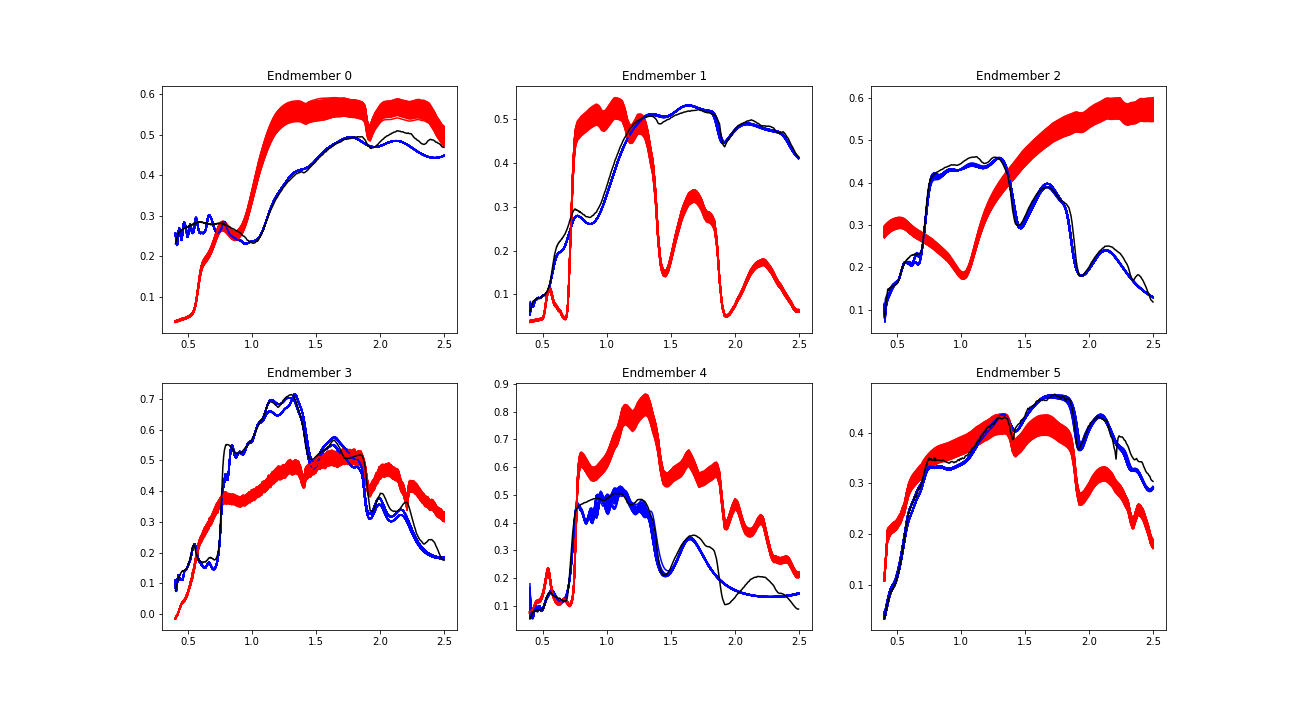
\includegraphics[width=\textwidth]{pictures/spectral_variab.png}
    \caption{Spatial spectral variability}
    \label{fig:variab}
\end{figure*}

Present result tables, images (ground truth/Janiczek/us), signatures (mean, max and min against ground truth and Janiczek).


\section{Conclusion}

This project presented a new approach to perform hyperspectral unmixing accounting for endmember variability. An explicit, physics-based model was combined with specific prior information on the elements of the problem, motivated by observations from the real world. This yielded a new formulation of the optimisation problem, that unfortunately wasn't differentiable. In order to take advantage of the great out-of-the-box and computationally efficient existing tools (automatic differentiation, GPU computing), and to bypass the difficulty of dealing directly with a complex model, we proposed a differentiable relaxation of the problem, along with a simple, classic algorithm to solve it. Furthermore, an implementation of the approach has been provided and is available online. Some experimentations were run to assess the relevance of the approach.

While some work has already been done, there are still a lot of perspectives to explore. First of all, to provide a good evaluation of the approach, more datasets should be considered. Additionally, there wasn't enough time to properly tune the algorithm, which is crucial considering the complexity of the problem. For instance, other minimization approach like Alternating Minimization could be considered. We could also use a way to automatically set the regularization parameters, as the experiments have highlighted a significant variability of the results in that respect.

%\section*{Acknowledgment}

\acks{I want to extend a sincere thank-you to my supervisor for this Research Project, Pierre-Antoine Thouvenin, for his great support and for proposing this subject. I also want to warmfully thank the unnamed heroes on Internet who share their knowledge when the code errors don't make any sense.}

%\section*{References}

% \bibliographystyle{IEEEtran}
\bibliography{unmixing,theory}


\section{Appendix}

\end{document}
